\chapter{Evaluation and project planning} \label{chap:evalProjPlan}

This milestone will focus on planning development steps and guidelines based on the evaluation of the previous milestone (see \ref{chap:proofConcept}).
A concrete plan will help develop a maintainable, quality application with a clear vision of a path towards the target goal.

\section{Evaluation}

\subsection{Project hosting platform}

The final project shall be open source and will be hosted on GitHub.
These decisions were made to allow external contributions, reach a niche target demographic, and to have access to freemium GitHub features, which are offered for free to open source projects.

GitHub was chosen over GitLab, the second best contendor, because the former platform offers better visibility and access - a crucial factor for reaching the target demographic.

\subsection{Technology stack}

\subsubsection{Frameworks}

The proof of concept application (see \ref{chap:proofConcept}) was developed in November 2018 using \nameref{sec:netFramework} and is hosted on GitLab\footnote{https://gitlab.com/hailstorm75/markdoc}. The resulting project shall be developed using \nameref{sec:netCore}, as it is the new development platform from Microsoft (see \ref{chap:overviewNET}). There are no reasons to stick with the old development platform.

\subsubsection{Languages}

C\# will be the primary programming language, as it is the dominant language for the \ref{gloss:dotnetlabel} platform.
F\# shall be used sparsly to fullfill a personal goal of exploring said languages capabilities.

\subsubsection{DI Framework}

For \ref{itm:di} the project shall use Autofac, which is a popular library with suitable features for this project. Chosing any other library would require investing additional time into learning how to use it; thus, no further analysis of available \ref{itm:di} frameworks was conducted.

\subsubsection{\ref{itm:gui} framework} \label{sec:guiFramework}

The \ref{gloss:dotnetlabel} ecosystem offers a rich selection of \ref{itm:gui} frameworks to chose from. What follows is a list of available frameworks during the time of analysis.

\textbf{From Microsoft:}
\begin{itemize}
    \item WinForms
    \item WPF
    \item UWP
    \item Xamarin
    \item Xamarin.Forms
    \item Blazor
\end{itemize}

\textbf{From the open source community:}
\begin{itemize}
    \item Avalonia UI
    \item UNO Platform
    \item Eto
\end{itemize}

The project is a developer tool for generating documentation; thus, it does not make sense to host it in the web, nor on mobile. This leaves only desktop \ref{itm:gui} frameworks. The only challenge is to pick one, which provides cross-platform capabilities. The cross-platform targets would be Windows OS, Linux-based distributions, and Mac OS.
Linux is the most crucial platform, as developers might want to run the tool on their \ref{itm:cicd} servers. It is possible that some of those servers would have a desktop interface, instead of just a \ref{itm:cli}.

At the time of the analysis, none of the frameworks provided by Microsoft qualified for the task. And even when the company released their new framework, .NET MAUI, it did not include support for Linux.

This leaves community built solutions.
Out of the three, Avalonia UI was the easiest to get up and running, and had a sizeable community, with extension libraries and other projects to support it. It is cross-platform and works primarily on desktop operating systems. The UNO Platform is very powerful on paper, and is both cross-platform and cross-device (desktop, mobile, web); however, after many attempts, it was not possible to even start the demo application. Eto is also a cross-platform framework, but it has a small community with few to no additional libraries to use.

Hence, the selected \ref{itm:gui} framework for the project is Avalonia UI.

\section{Development planning}

\subsection{Project architecture} \label{sec:projectArchitecture}

Applying \ref{itm:solid} principles helped invision an architecture of a maintainable and extendable application.
The primary principle, Single-responsibility, helps separate operations within the application into key parts (see \ref{sec:projectComponents}), where each part plays its individual key role in the application.

The \textit{Dependency inversion} principle is applied to inch closer to an extensible application. Every key dependency is decoupled with an interface, allowing for the \textit{\ref{itm:di}} design pattern; thus, parts of the application can be swapped, and even rearranged at will. This factor allows for flexible extensibility and fullfills the Open-closed principle from \ref{itm:solid}.

Implementing such an architecture would require defining said decoupled interfaces first.
The next step would be to create specific implementations of said interfaces. E.g., \textit{Diagram Generator} would be the interface, while \textit{PlatUML Diagram generator}, or \textit{MermaidJS Diagram generator} would be the specific implementations deriving from said interface.

Specific implementations of an interface will be referred to as \textbf{components}. Given that there might be various implementations of one interface, a group of specific implementations would be referred to as a \textbf{plugin}. A user would install only those plugins that they need for their task. And a developer would create a custom plugin by grouping specific components that either already exist, or they would have written themselves.

\begin{figure}[H]
    \centering
    \caption{Application architecture}
    \label{fig:applicationArchitecture}
    \tikzset{every picture/.style={line width=0.75pt}} %set default line width to 0.75pt
        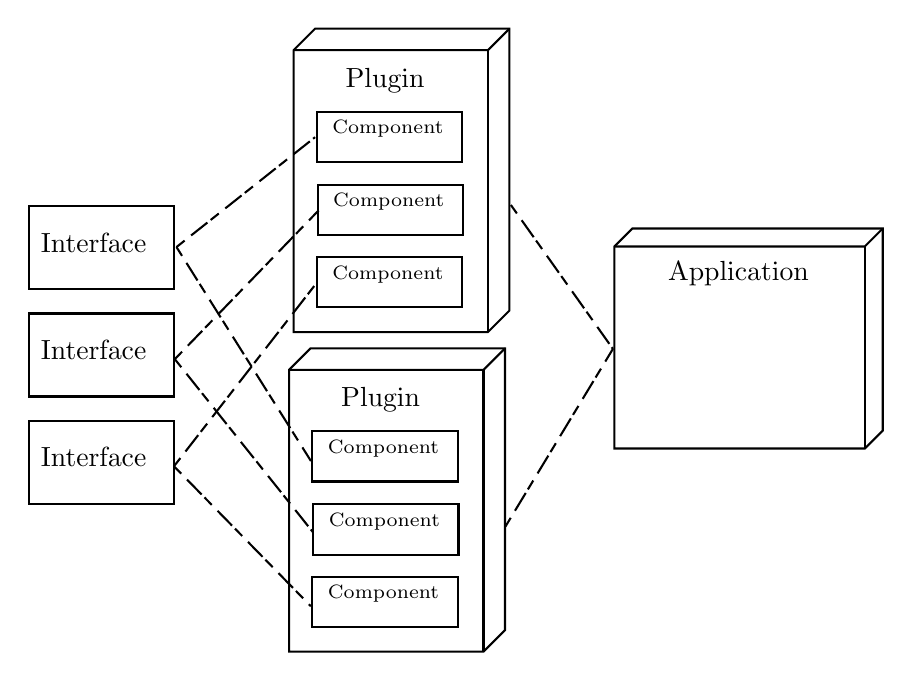
\begin{tikzpicture}[x=0.75pt,y=0.75pt,yscale=-1,xscale=1]
        %uncomment if require: \path (0,322); %set diagram left start at 0, and has height of 322

        %Shape: Cube [id:dp6966791057530186] 
        \draw   (136.8,15.75) -- (147.15,5.4) -- (240.8,5.4) -- (240.8,141.2) -- (230.45,151.55) -- (136.8,151.55) -- cycle ; \draw   (240.8,5.4) -- (230.45,15.75) -- (136.8,15.75) ; \draw   (230.45,15.75) -- (230.45,151.55) ;
        %Shape: Rectangle [id:dp5584628563018248] 
        \draw   (148,45.4) -- (218,45.4) -- (218,69.55) -- (148,69.55) -- cycle ;
        %Shape: Rectangle [id:dp4204128193938954] 
        \draw   (148.4,80.6) -- (218.4,80.6) -- (218.4,104.75) -- (148.4,104.75) -- cycle ;
        %Shape: Rectangle [id:dp08451759114862534] 
        \draw   (148,115.4) -- (218,115.4) -- (218,139.55) -- (148,139.55) -- cycle ;

        %Shape: Cube [id:dp4027980103737905] 
        \draw   (134.67,169.75) -- (145.02,159.4) -- (238.67,159.4) -- (238.67,295.2) -- (228.32,305.55) -- (134.67,305.55) -- cycle ; \draw   (238.67,159.4) -- (228.32,169.75) -- (134.67,169.75) ; \draw   (228.32,169.75) -- (228.32,305.55) ;
        %Shape: Rectangle [id:dp9964695428644907] 
        \draw   (145.87,199.4) -- (215.87,199.4) -- (215.87,223.55) -- (145.87,223.55) -- cycle ;
        %Shape: Rectangle [id:dp7687242463256714] 
        \draw   (146.27,234.6) -- (216.27,234.6) -- (216.27,258.75) -- (146.27,258.75) -- cycle ;
        %Shape: Rectangle [id:dp8340195335075327] 
        \draw   (145.87,269.4) -- (215.87,269.4) -- (215.87,293.55) -- (145.87,293.55) -- cycle ;

        %Shape: Rectangle [id:dp04284178514770831] 
        \draw   (9.2,194.2) -- (79.2,194.2) -- (79.2,234.2) -- (9.2,234.2) -- cycle ;

        %Shape: Rectangle [id:dp547256482285905] 
        \draw   (9.2,142.6) -- (79.2,142.6) -- (79.2,182.6) -- (9.2,182.6) -- cycle ;

        %Shape: Rectangle [id:dp058814608034839067] 
        \draw   (9.2,91) -- (79.2,91) -- (79.2,131) -- (9.2,131) -- cycle ;

        %Straight Lines [id:da06998801958778844] 
        \draw  [dash pattern={on 3.75pt off 3pt on 7.5pt off 1.5pt}]  (80.4,110.6) -- (147.17,57.67) ;
        %Straight Lines [id:da6710004482385108] 
        \draw  [dash pattern={on 3.75pt off 3pt on 7.5pt off 1.5pt}]  (80.4,110.6) -- (145.17,213.67) ;
        %Straight Lines [id:da174380515876845] 
        \draw  [dash pattern={on 3.75pt off 3pt on 7.5pt off 1.5pt}]  (79.6,164.6) -- (148.83,93) ;
        %Straight Lines [id:da6199004493954201] 
        \draw  [dash pattern={on 3.75pt off 3pt on 7.5pt off 1.5pt}]  (79.6,164.6) -- (146.17,248) ;
        %Straight Lines [id:da7585298700928582] 
        \draw  [dash pattern={on 3.75pt off 3pt on 7.5pt off 1.5pt}]  (79.2,216.2) -- (147.83,128) ;
        %Straight Lines [id:da40931164919739227] 
        \draw  [dash pattern={on 3.75pt off 3pt on 7.5pt off 1.5pt}]  (79.2,216.2) -- (145.17,283.67) ;
        %Shape: Cube [id:dp29755236766759063] 
        \draw   (291.33,110.33) -- (300,101.67) -- (420.67,101.67) -- (420.67,199) -- (412,207.67) -- (291.33,207.67) -- cycle ; \draw   (420.67,101.67) -- (412,110.33) -- (291.33,110.33) ; \draw   (412,110.33) -- (412,207.67) ;
        %Straight Lines [id:da8639799165876028] 
        \draw  [dash pattern={on 3.75pt off 3pt on 7.5pt off 1.5pt}]  (241.5,90.33) -- (290.67,159.67) ;
        %Straight Lines [id:da254713623135423] 
        \draw  [dash pattern={on 3.75pt off 3pt on 7.5pt off 1.5pt}]  (238.83,245.33) -- (290.67,159.67) ;

        % Text Node
        \draw (151.87,272.2) node [anchor=north west][inner sep=0.75pt]   [align=left] {{\scriptsize Component}};
        % Text Node
        \draw (152.27,237.4) node [anchor=north west][inner sep=0.75pt]   [align=left] {{\scriptsize Component}};
        % Text Node
        \draw (151.87,202.2) node [anchor=north west][inner sep=0.75pt]   [align=left] {{\scriptsize Component}};
        % Text Node
        \draw (158.27,176.8) node [anchor=north west][inner sep=0.75pt]   [align=left] {Plugin};
        % Text Node
        \draw (13.6,205.6) node [anchor=north west][inner sep=0.75pt]   [align=left] {Interface};
        % Text Node
        \draw (13.6,154) node [anchor=north west][inner sep=0.75pt]   [align=left] {Interface};
        % Text Node
        \draw (13.6,102.4) node [anchor=north west][inner sep=0.75pt]   [align=left] {Interface};
        % Text Node
        \draw (315.73,116.13) node [anchor=north west][inner sep=0.75pt]   [align=left] {Application};
        % Text Node
        \draw (160.4,22.8) node [anchor=north west][inner sep=0.75pt]   [align=left] {Plugin};
        % Text Node
        \draw (154,48.2) node [anchor=north west][inner sep=0.75pt]   [align=left] {{\scriptsize Component}};
        % Text Node
        \draw (154.4,83.4) node [anchor=north west][inner sep=0.75pt]   [align=left] {{\scriptsize Component}};
        % Text Node
        \draw (154,118.2) node [anchor=north west][inner sep=0.75pt]   [align=left] {{\scriptsize Component}};
    \end{tikzpicture}
\end{figure}

\subsection{Interfaces} \label{sec:projectComponents}

The primary principle, Single-responsibility, separated operations within the application into the following key parts:
\begin{itemize}
    \item Member provider
    \item Documentation provider
    \item Composer
    \item Element provider
    \item Diagram generator
    \item Linker
    \item Printer
\end{itemize}

\subsubsection{Member provider}

The member provider will be responsible for loading type and member data from a given collection of sources into a collection of a defined data structure.
This collection will then be provided to the consumer of this key part via the relevant interface.
A concrete implementation of the interface would define the source type and the method for processing said source.

\subsubsection{Documentation provider}

The documentation provider will be responsible for loading documentation for specific types and members from a given collection of sources and mapping said documentation to the relevant types and members.
The map will then be available for querying to consumers of this key part via the relevant interface.
A concrete implementation of the interface would define the source type and the method for processing said source.

\subsubsection{Element provider} \label{sec:elementProvider}

The element provider will be responsible for providing structural elements for the visual representation of the generated documentation. Such elements would include:
\begin{description}
    \item[Text] regular text without any formatting
    \item[Formatted text] text with formatting, e.g. bold, italic, code
    \item[Lists] numbered, bullet, term lists
    \item[Tables] headered tables
    \item[Sections] content separators with headings containing all of the above
    \item[Pages] content separators containing sections
\end{description}

Consumers of this provider would create required elements via the relevant interface.
A concrete implementation of the interface would define how said elements are to be represented, e.g. \ref{gloss:markdown}, \ref{itm:html}, \LaTeX.

\subsubsection{Diagram generator}

The diagram generator will be primarily responsible for creating inheritance diagrams for provided types. Additional diagraming features such as a class structure, EF Core relational model, etc. won't be part of this thesis.
A concrete implementation of this interface would define how said diagrams will be delivered, e.g. as text, or as a link to a file.
In case of text, they could be delivered as \ref{gloss:asciiart}, a PlantUML or MermaidJS diagrams.

\subsubsection{Linker}

The linker interface will be responsible for creating links between resolved types, and anchor links to sections of documentation pages.
A concrete implementation of this interface would define how said links are to be generated to fit the target platform, e.g. GitHub and GitLab have different link formats.

\subsubsection{Composer} \label{sec:composer}

The composer interface will be repsonsible for iterating through the resolved data, combining and filtering it, then composing it into section and page elements from the respective provider (see \Nameref{sec:elementProvider}).
Specific implementations of this interface would define the result of the composition.

\subsubsection{Printer}

The printer interface will be responsible for exporting the composed elements (see \Nameref{sec:composer}) into the desired format.
Specific implementations will define how and where the result is exported.

\subsection{\ref{itm:gui} application}

Based on the developer needs analysis (see \ref{sec:whatdouserswant}), users of such a tool expect a \ref{itm:cli} application. However, configuring such an extensible tool via the command line can be overwhelming.
This can be solved by providing a \ref{itm:gui} application for creating configurations, testing them, and later creating a \ref{itm:cli} for executing the generated configurations in, for example, a \ref{itm:cicd} pipeline.
To summarize, the purpose of this application would be to provide

\subsection{Plugin structure}

As described in \Nameref{sec:projectArchitecture}, plugins will wrap a combination of specific components that define the plugin's functionality.
Since components are supposed to be independant from one another, they must be individually configured.
Thus, the plugin must provide configuration steps for the application to consume, and display to the user.
The internal architecture of the plugin is up-to its developer, the only mandatory conditions are:
\begin{itemize}
    \item Provide configuration steps for the components
    \item Provide an endpoint for executing the configured components
\end{itemize}

\subsection{Development stages} \label{sec:developmentStages}

Since the project is divided into interfaces, components, plugins, and the \ref{itm:ui} application, it makes sense to define development steps based on said architecture.

\begin{enumerate}
    \item \label{num:stage1} Define the shared interfaces
    \item \label{num:stage2} Create the reflection-based member resolver component
    \item \label{num:stage3} Create the \ref{itm:xml} documentation resolver component
    \item \label{num:stage4} Create the Git link resolver component
    \item \label{num:stage5} Create the \ref{gloss:markdown} elements component
    \item \label{num:stage6} Create the MermaidJS diagram generator component
    \item \label{num:stage7} Create the composer component
    \item \label{num:stage8} Create the printer component
    \item \label{num:stage9} Create the \ref{itm:gui} application
    \item \label{num:stage10} Create the \ref{gloss:markdown} plugin
\end{enumerate}

Completing all of these steps will be the solution to the goal of this thesis.